%% ==============================================================
%% WARNING! ENGLISH SPEAKING AUTHORS SHOULD READ gretsien.tex
%%          FILE INSTEAD
%% ==============================================================
%% EXEMPLE DE CONTRIBUTION AU GRETSI
%% POUR LES UTILISATEURS FRANCOPHONES DE LaTeX2e
  \documentclass{gretsi}
%% Selectionnez ensuite les paquets que vous utilisez,
%% par suppression ou adjonction d'un caractere %
%% en debut de ligne (mise en commentaire).
%% --------------------------------------------------------------
%% UTILISATION DE CARACTERES ACCENTUES AU CLAVIER ?
%% (le codage du clavier depend du systeme d'exploitation)
% \usepackage[applemac]{inputenc} % MacOS
% \usepackage[ansinew]{inputenc}  % Windows ANSI
% \usepackage[cp437]{inputenc}    % DOS, page de code 437
% \usepackage[cp850]{inputenc}    % DOS, page de code 850
% \usepackage[cp852]{inputenc}    % DOS, page de code 852
% \usepackage[cp865]{inputenc}    % DOS, page de code 865
% \usepackage[latin1]{inputenc}   % UNIX, codage ISO 8859-1
% \usepackage[decmulti]{inputenc} % VMS
% \usepackage[next]{inputenc}
% \usepackage[latin2]{inputenc}
% \usepackage[latin3]{inputenc}
%% --------------------------------------------------------------
%% REGLES DE TYPOGRAPHIE FRANCAISES ?
 \usepackage[english,french]{babel}   % "babel.sty" + "french.sty"
% \usepackage[english,francais]{babel} % "babel.sty"
 % \usepackage{french}                  % "french.sty"
 \usepackage[utf8]{inputenc}
 \usepackage{times}			% ajout times le 30 mai 2003
\usepackage{amsmath}
\usepackage{amssymb}
\usepackage{graphics}
\usepackage{algorithm2e}
\SetKwRepeat{Do}{Faire}{Tant que}
\graphicspath{{images/}}
\hyphenation{fail-libles}
\usepackage{natbib} 

%% --------------------------------------------------------------
%% CODAGE DE POLICES ?
%% Si votre moteur Latex est francise, il est conseille
%% d'utiliser le codage de police T1 pour faciliter la c\'esure,
%% si vous disposez de ces polices (DC/EC)
% \usepackage[T1]{fontenc}
%% ==============================================================

\titre{Impact du bruit synaptique sur les performances des \\ réseaux de cliques neurales}

\auteur{\coord{Eliott}{Coyac}{},
        \coord{Vincent}{Gripon}{},
    \coord{Charlotte}{Langlais}{},
    \coord{Claude}{Berrou}{}}

\adresse{\affil{}{Lab-STICC \\ Télécom Bretagne, Brest }}

%% Si tous les auteurs ont la m\^eme adresse %%%%%%%%%%%%%%%%%%%%%%%%%%%%%%%%%%%%
%                                                                             %
%   \auteur{\coord{Michel}{Dupont}{},                                         %
%           \coord{Marcel}{Dupond}{},                                         %
%           \coord{Michelle}{Durand}{},                                       %
%           \coord{Marcelle}{Durand}{}}                                       %
%                                                                             %
%   \adresse{\affil{}{Laboratoire Traitement des Signaux et des Images \\     %
%     1 rue de la Science, BP 00000, 99999 Nouvelleville Cedex 00, France}}   %
%                                                                             %
%%%%%%%%%%%%%%%%%%%%%%%%%%%%%%%%%%%%%%%%%%%%%%%%%%%%%%%%%%%%%%%%%%%%%%%%%%%%%%%

\email{prénom.nom@telecom-bretagne.eu}

\resumefrancais{Les réseaux de neurones s'inspirent du fonctionnement et de la structure du cerveau, et l'argument de la plausibilité biologique est souvent utilisé pour défendre ou critiquer un modèle par rapport à un autre. La littérature neurobiologique nous renseigne sur le fait que le cerveau est un système bruité, dans lequel les composants et leurs connexions sont non fiables. Pourtant, le comportement des réseaux de neurones face à ce bruit a rarement été étudié. Ce papier propose un modèle de bruit cérébral et analyse son impact sur les performances des réseaux de cliques neurales. Nous montrons que le bruit peut les améliorer, notamment en évitant des minima locaux. Nous analysons également l'impact de ce bruit sur les performances des réseaux de Hopfield.}

\resumeanglais{Artificial neural networks are inspired by biological neural networks present in the brain, and biological plausibility is often used as an argument to validate or criticize a neural network proposal. However, the brain is a system with a lot of interferences and the behaviour of neural networks towards this noise is not often studied. This paper first suggests a way to represent noise inside the brain, and then studies how Neural Clique networks respond to that noise. It is shown that they can actually improve performance by avoiding local minima using the noise. A comparison with Hopfield networks is also given, responding to the same noise.}

\begin{document}
\maketitle

\section{Introduction}

TODO: citer le papier de François.

Le cerveau a inspiré de nombreux modèles de réseaux de neurones. Parmi eux, les réseaux de Hopfield~\cite{}, les machines de Boltzmann~\cite{}, les réseaux de Willshaw~\cite{} et plus récemment les réseaux de cliques neurales~\cite{} implémentent des mémoires associatives. Ces mémoires, par contraste avec les mémoires indexées classiques, permettent d'accéder à un élément d'information stocké à partir d'une fraction de son contenu. Parmi les modèles de réseaux de neurones, deux grandes familles s'opposent. La première considère que l'information est stockée dans le poids des synapses reliant les neurones (e.g. Hopfield, Boltzmann\dots). La seconde propose que l'information est stockée dans l'existence de connexions formant des motifs graphiques (e.g. Willshaw, réseaux de cliques neurales\dots).

Réciproquement, ces réseaux ont souvent été utilisés pour modéliser la mémoire cérébrale. Des publications de la littérature neurobiologique~\cite{} nous renseignent sur le fait que les neurones biologiques et leurs connexions sont non fiables. Les réseaux de neurones actuels s'inspirent du cerveau et de la structure possible des neurones, en prenant en compte la loi de Hebb ou de Huxley, mais peu s'intéressent à l'environnement de ces neurones - et le bruit provoqué par cet environnement. Le cerveau étant un système biologique, ses composantes sont faillibles et des perturbations sont présentes.

Dans ce papier, nous introduisons un modèle de bruit s'appliquant aux réseaux de neurones artificiels et s'inspirant du cerveau. Nous analysons l'impact de ce bruit sur deux modèles de mémoires associatives : les réseaux de Hopfield et les réseaux de cliques neurales. Pour ce dernier, nous montrons que le bruit peut aider les performances en évitant les minima locaux.

Le reste du papier est organisé de la manière suivante. La partie 2 introduit un modèle de bruit pour les réseaux de neurones artificiels. La partie 3 présente les modèles de mémoires associatives de Hopfield et les réseaux de cliques neurales. La partie 4 étudie l'impact du bruit proposé sur les performances de ces modèles. La partie 5 conclue.

\section{Modèle de bruit dans le cerveau}

Le cerveau est un système non fiable. Il y a plusieurs raisons à cela, à plusieurs niveaux, des interférences produites par des neurones s'activant spontanéments jusqu'à des causes chimiques. Dans ce papier nous nous intéressons à la faillibité des synapses (\citep{zador1998impact}). Chaque neurone possède un axone, s'attachant à de nombreux autres neurones par le biais de synapses. Un axone se connecte à un neurone par plusieurs synapses, et les synapses libèrent parfois des neurotransmetteurs quand le neurone d'origine est stimulé. La probabilité qu'un synapse libère des neurotransmetteurs peut varier de 20\% à 80\% \citep{branco2009probability}.

Nous proposons un modèle où chaque neurone est connecté à un autre neurone par $n_{syn}$ synapses. Chaque synapse est munie d'une probabilité $p_{rel}$ de libérer des neurotransmetteurs lorsqu'elle est stimulée. Pour simplifier, nous prenons l'hypothèse que ces probabilités sont indépendantes. Par conséquent, lorsqu'un neurone émet un signal, les neurones auxquels il est connecté reçoivent une stimulation suivant une loi binomiale $B(n_{syn}, p_{rel})$.

\section{Mémoires associatives}

\subsection{Réseaux de Hopfield}

Un réseau de Hopfield~\cite{} est porté par un graphe complet reliant $n$ neurones. Un tel graphe peut stocker des messages binaires ($\{-1,1\}$) de longueur $n$. Chaque neurone est étiquetté de 1 à $n$, de sorte que un message à stocker correspond à une valeur $-1$ ou $1$ attribuée à chaque neurone du réseau.

Pour stocker un message, le réseau de Hopfield incrémente le poids des connexions reliant des neurones qui observent la même valeur, tandis qu'il décrémente ceux des connexions reliant des neurones observant des valeurs différentes.

Formellement, si $\mathcal{M}$ est l'ensemble des messages binaires à stocker, alors la matrice d'adjacence $W(\mathcal{M})$ du réseaux de Hopfield correspondant est :
\begin{equation}
 W(\mathcal{M}) \triangleq \sum_{m\in\mathcal{M}}{m \cdot m^{\top}}\;,
 \end{equation}
 où $m^\top$ est la transposée de $m$.

 Le réseau de Hopfield peut retrouver un message stocké à partir d'une fraction de son contenu en entrée. Nous obtenons un \textit{message effacé} $\tilde{m}$ à partir du message $m$ en remplaçant certaines de ses coordonnées par $0$.

 Pour retrouver $m$ à partir de $\tilde{m}$ et de $W(\mathcal{M})$, les réseaux de Hopfield utilisent l'algorithme itératif suivant :
 \begin{algorithm}
   \KwData{W(\mathcal{M}),\tilde{m}}
   v \leftarrow \tilde{m}\\
   \Do{$v \not= w$}{
     w \leftarrow v\\
     v \leftarrow sgn(W(\mathcal{M})\cdot w)\\
   }
   Rendre $v$\;
  \caption{Algorithme pour retrouver un message à partir d'une version effacée dans un réseau de Hopfield. La fonction $sgn$ est la fonction qui à un entier associe son signe.}
\end{algorithm}

\subsection{Réseaux de cliques neurales}

Un réseau de cliques neurales~\cite{} est porté par un graphe composé de $c$ parties contenant chacune $\ell$ fanaux\footnote{Les auteurs de~\cite{} utilisent le terme ``fanal'' au lieu de ``neurone'' car un fanal représente une assemblée de neurones (microcolonne).}. Contrairement aux réseaux de Hopfield, les connexions ne sont pas pondérées. Une information est alors représentée dans le réseau sous la forme d'un motif complètement interconnecté (clique).

Formellement, les messages pouvant être stockés dans un tel réseau sont des vecteurs binaires ($\{0,1\}$) de longueur $c\ell$ pouvant être découpés en $c$ blocs de $\ell$ coordonnées, de sorte que dans chaque bloc n'apparaisse qu'un seul $1$. De tels messages sont typiquement obtenus en utilisant un codage disjonctif complet~\cite{}.

La matrice d'adjacence du réseau de cliques neurales obtenu après stockage des messages contenus dans l'ensemble $\mathcal{M}$ est :
\begin{equation}
\mathfrak{W}(\mathcal{M}) \triangleq \max_{m\in\mathcal{M}}{m \cdot m^{\top}}\;,
\end{equation}
où $\max$ est appliqué à chaque coefficient de la matrice indépendamment.

Dans le contexte des réseaux de cliques neurales, on appelle message effacé $\tilde{m}$ une modification d'un message stocké $m$ où certains 1 ont été transformés en 0.

Nous introduisons la fonction de \textit{winner-takes-all} local suivante :
\begin{equation}
u(v)_i \triangleq \left\{\begin{array}{ll} 1&\text{ si } v_i \text{ est la valeur maximale dans le bloc }\\&\text{où se trouve la coordonnée } i\\0&\text{ sinon}\end{array}\right.
\end{equation}
  
Pour retrouver $m$ à partir de $\tilde{m}$ et $\mathfrak{W}(\mathcal{M})$, on utilise l'algorithme suivant :

 \begin{algorithm}
   \KwData{\mathfrak{W}(\mathcal{M}),\tilde{m}}
   v \leftarrow \tilde{m}\\
   \Do{$v \not= w$}{
     w \leftarrow v\\
     v \leftarrow u(W(\mathcal{M})\cdot w)\\
   }
   Rendre $v$\;
   \caption{Algorithme pour retrouver un message à partir d'une version effacée dans un réseau de cliques neurales.}
   \label{alg:cliques}
\end{algorithm}

\section{Impact du bruit sur les performances}

\subsection{Cas des réseaux de Hopfield}

La Figure~\ref{fig:hopfield} montre la comparaison des performances obtenues par un réseau de Hopfield selon si le bruit introduit en partie 2 est pris en compte ou non. Ces réseaux contiennent $n=2048$ neurones et sont capables de stocker environs 100 messages de façon à pouvoir les retrouver lorsque la moitié des coordonnées sont effacées. Le paramètres pour le modèle de bruit sont : $n_{syn} = 10$ et $p_{rel} = 50\%$.

\begin{figure}[ht!]
\begin{center}
\resizebox{88mm}{!}{
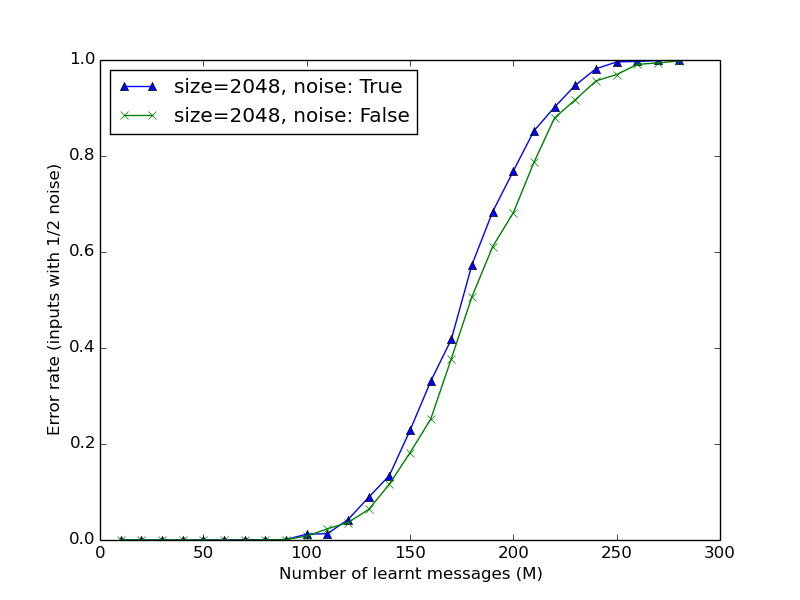
\includegraphics{hopfield-1}}
\end{center}
\legende{Résultats simulés sur un réseau de Hopfield de 2048 nœuds, avec ou sans bruit et $\tfrac{1}{2}$ des données effacées.}
\label{fig:hopfield}
\end{figure}

Nous observons un léger déclin en performance lorsque le bruit est appliqué. Le fait que les performances ne soient pas impactées de façon significative est probablement d\^u au grand nombre de signaux s'échangeant entre les nœuds, moyennant les effets du bruit.

\subsection{Réseaux de cliques neurales}

Pour introduire le modèle de bruit dans le réseau de cliques neurales, chaque connexion avec un nœud activé ajoute au score la valeur d'une variable aléatoire suivant la loi binomiale $B(n_{syn}, p_{rel})$. 

\subsubsection{Après une itération}

Dans les paragraphes suivant, nous analysons la probabilité de retrouver un message partiellement effacé après une itération de l'algorithme~\ref{alg:cliques}.

Soit un réseau à cliques ayant stocké $M$ messages. Notons $c_k$ le nombre de coordonnées non effacées (1 non transformés en 0) et $c_e$ le nombre de coordonnées effacées ($c_e = c-c_k$). Les performances dépendent grandement de la densité du réseau, c'est-à-dire la rapport entre le nombre de connexions utilisées et le nombre de connexions maximum. Dans le cas où les messages stockés sont indépendamment et uniformément distribués, celle-ci est définie par~\cite{} :
\begin{equation}
d = 1-\left(1-\frac{1}{\ell^2}\right)^M.
\end{equation}

Considérons un bloc effacé dans le message~\tilde{m}. Soit $s_0$ la coordonnée ayant été effacée et $n_{s_{0}}$ son score. Soit $s$ un nœud incorrect et $n_s$ son score. Le score d'un nœud s'apparente au nombre de synapses qui libèrent des neurotransmetteurs à destination du neurone représentant ce nœud. Donc un nœud connecté à $i$ autres nœuds actifs peut obtenir un score entre $0$ et $i \cdot n_{syn}$. Le nœud correct est bien s\^ur connecté aux $c_k$ autres nœuds initiaux. Donc pour la première itération, pour $x$ de $0$ à $n_{syn} \cdot c_k$, nous avons:

\begin{equation}
\begin{split}
P(n_{s_0}=x) & = P\left(B(n_{syn}\cdot c_k, p_{rel})=x\right)\\
             & = pmf(x, n_{syn}\cdot c_k, p_{rel})
\end{split}
\end{equation}

En effet la somme de $c_k$ variables aléatoires suivant une loi binomiale $B(n_{syn}, p_{rel})$ est $B(n_{syn}\cdot c_k, p_{rel})$. Nous choisissons aussi de noter la fonction de masse de la loi binomiale $pmf$. Nous avons la fonction de probabilité du score que le nœud correct obtient. Maintenant, pour déterminer cette fonction pour un nœud incorrect, nous devons tout d'abord savoir à combien de nœuds initiaux ce nœud est connecté. On trouve:

\begin{equation}
P_E(i) = \binom{c_k}{i} d^i (1-d)^{{c_k}-i}.
\end{equation}

où $P_E(i)$ représente la probabilité qu'un nœud incorrect soit connecté à $i$ nœuds initiaux.
%Indeed, the probability of not being connected to any of the known fanals is $(1-d)^{c_k}$ and the probability of being connected to all the known fanals is $d^{c_k}$. The probability of being connected to only a specific known fanal is $(1-d)^{c_k-1}d$, and to be solely connected to any one of the known fanals is $c_k \cdot (1-d)^{c_k-1}d$.

Ainsi, la probabilité qu'un nœud incorrect obtienne un score $x_0$ pour tout $ 0 \leq x_0 \leq n_{syn} \cdot c_k $ est:

\begin{equation}
\begin{split}
P(n_s=x_0) & = \sum_{i=0}^{c_k} P_E(i)\ pmf(x_0, n_{syn} \cdot i, p_{rel})\\
P(n_s\leq x_0) & = \sum_{x=0}^{x_0}\sum_{i=0}^{c_k} P_E(i)\ pmf(x, n_{syn}\cdot i, p_{rel})
\end{split}
\end{equation}

à l'aide de ces formules, nous pouvons écrire la probabilité qu'un nœud soit parmi les nœuds avec le plus haut score dans la grappe:

\begin{equation}
P_{succ}(s_0) = \sum_{x_0=0}^{n_{syn}\cdot c_k}P(n_{s_0}=x_0) P(n_s \leq x_0) ^ {l-1}.
\end{equation}

La probabilité de succès globale, c'est-à-dire que pour toutes les grappes le nœud correct soit parmi les nœuds avec le plus haut score de la grappe est $P_{succ} = P_{succ}(s_0)^{c_e}$. Le taux d'erreur est $1-P_{succ}$.

Néanmoins, cette approche n'est pas assez stricte. à l'itération finale, un nœud unique par grappe a besoin d'\^etre choisi, pour obtenir un résultat final comportant $c$ nœuds. C'est-à-dire, lorsque plusieurs nœuds partagent le plus haut score dans une grappe, un nœud doit \^etre choisi. Il y a une chance $\frac{1}{k+1}$ de trouver le bon nœud, si $k$ est le nombre de nœuds incorrects partageant le plus haut score avec le nœud correct.

Pour prendre cela en compte, $P_{succ}(s_0)$ est réécrite. Tout d'abord on introduit la probabilité de choisir le bon nœud si son score est $x_0$:

\begin{equation}
P_{succ}(s_0, n_{s_0}=x_0) = \sum_{k=0}^{l-1}\frac{1}{k+1} \binom{l-1}{k} P(n_s = x_0)^k P(n_s < x_0)^{(l-1-k)}
\end{equation}

et

\begin{equation}
P_{succ}(s_0) = \sum_{x_0=0}^{n_{syn}\cdot c_k}P(n_{s_0}=x_0) P_{succ}(s_0, n_{s_0}=x_0).
\end{equation}

Le taux de succès global, c'est-à-dire que dans toutes les grappes le nœud correct est choisi, est $P_{succ} = P_{succ}(s_0)^{c_e}$. Le taux d'erreur est naturellement :

\begin{equation}
P_{err} = 1-P_{succ}.
\end{equation}

\begin{figure}[ht!]
\begin{center}
\resizebox{88mm}{!}{
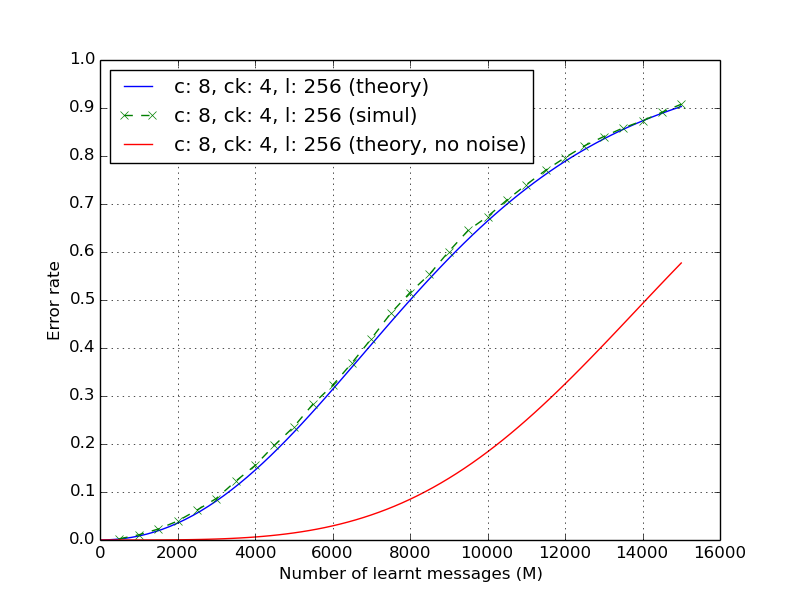
\includegraphics{weak}}
\end{center}
\legende{Résultats théoriques et simulés après une itération avec $\chi=8, c_k=4, l=256$.}
\label{fig:f1}
\end{figure}

Ces formules ont été testées par une simulation, et comme montré sur la figure~\ref{fig:f1} les deux courbes théorique et simulée sont très proches. La troisième courbe, avec le plus bas taux d'erreur, est la courbe de référence quand le bruit est absent.

\subsubsection{Après plusieurs itérations}

\paragraph{Condition d'arr\^et} Il s'agit d'abord de définir une condition d'arr\^et pour l'algorithme. En effet, le bruit implique une absence d'état stable dans l'algorithme et un nouveau critère d'arrêt pour l'algorithme doit être choisi. On choisit de limiter le nombre d'itérations à 100 pour limiter le temps d'exécution. De plus, l'algorithme s'arrête si le résultat est stable après $k$ itérations où $k$ est choisi au préalable. La figure~\ref{fig:stable-test} montre le taux d'erreurs pour différentes valeurs de $k$. Pour un nombre très petit de messages, $k=4$ est meilleur, mais ensuite $k=3$ est préférable jusqu'à un taux d'erreur de $20\%$.

\begin{figure}[ht!]
\begin{center}
\resizebox{88mm}{!}{
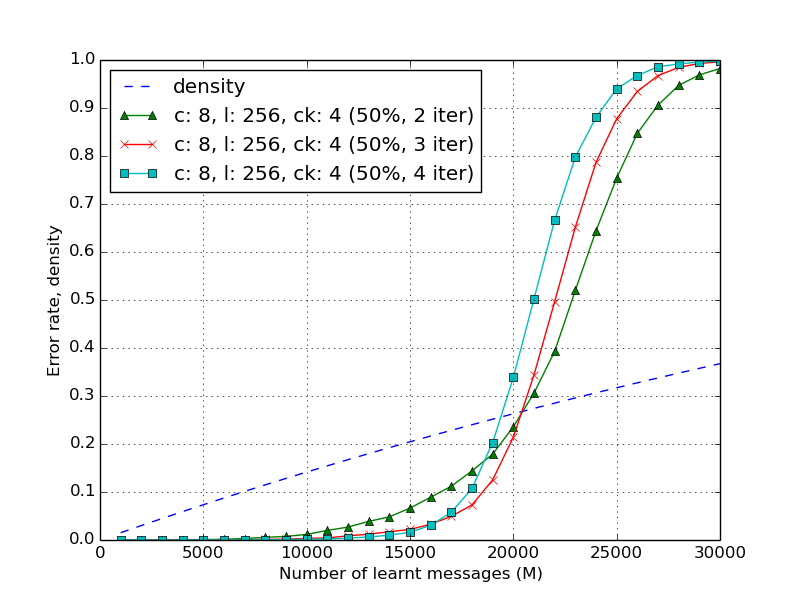
\includegraphics{stable-test}}
\end{center}
\legende{Résultats simulés avec $p_{rel}=0.5$ et $\chi=8, c_k=4, l=256$, s'arrêtant après 2, 3 ou 4 itérations stables.}
\label{fig:stable-test}
\end{figure}

Actuellement, nous sommes seulement capable de produire une formule mathématique pour le taux d'erreurs après une itération. Pour plusieurs itérations, seules des simulations nous permettent d'obtenir les résultats. 

\begin{figure}[ht!]
\begin{center}
\resizebox{88mm}{!}{
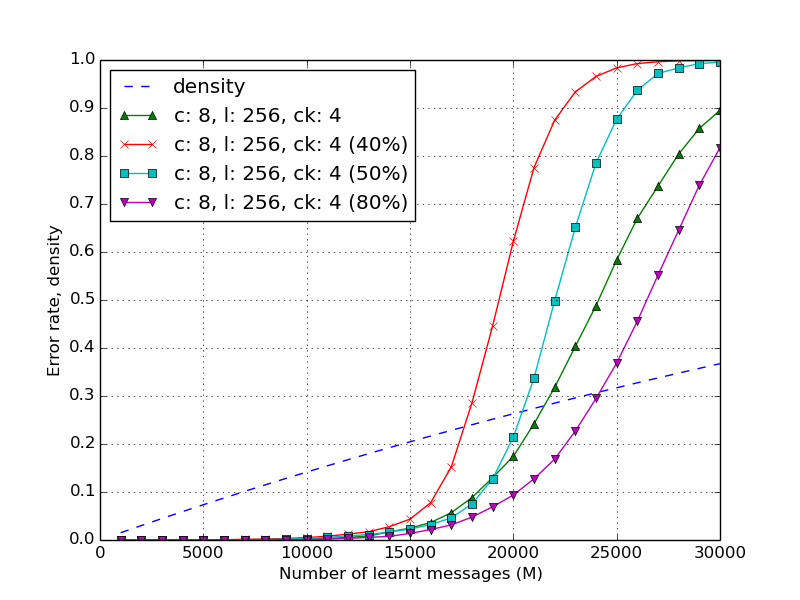
\includegraphics{full-mult}}
\end{center}
\legende{Résultats simulés sur plusieurs itérations avec $p_{rel}$ allant de $0.4$ à $0.8$.}
\label{fig:full-mult}
\end{figure}

Comme la figure~\ref{fig:full-mult} le montre, le bruit peut avoir des effets bénéfiques pour le réseau de neurones à cliques. Pour $p_{rel} = 0.5$, il y a une amélioration pour les taux d'erreurs en dessous de $10\%$. Pour $p_{rel} = 0.8$, il y a une nette amélioration pour tous les taux d'erreurs envisageables.

Ces résultats peuvent être attribués au fait d'éviter les minima locaux gr\^ace au bruit, de la même manière que l'algorithme du recuit simulé.



\section{Discussion}

Certains critères dans ce papier ont été choisis de manière arbitraire, comme le nombre de contacts synaptiques par connexion entre deux neurones ou la probabilité d'un synapse de libérer des neurotransmitteurs. $50\%$ ou $80\%$ pour cette probabilité peut sembler un chiffre élevé, mais d'après \citep{branco2009probability} cette probabilité s'ajuste en fonction des besoins. De plus, choisir $n_{syn}=20$ au lieu de $10$ diminue la variance du bruit de la même manière qu'augmenter la probabilité de libérer des neurotransmitteurs. Enfin, l'hypothèse d'évènements indépendants dans le temps a été faite dans ce papier, mais il est facile d'imaginer qu'un synapse a plus de probabilité de libérer des neurotransmitteurs pour une stimulation s'il n'en a pas relaché à la stimulation précédente, et inversement. Ceci réduirait aussi la variance du bruit.


\begin{itemize}
\item \emph{Todo: } Tester avec $n_{syn}=20$
\end{itemize}



\bibliographystyle{alpha}
\bibliography{research}

\end{document}
